% Xinzhi: This tikz file is automatically generated by mathcha editor, link: https://www.mathcha.io/editor/Q2WoQCVmFEdfqZCK6qPjLteWJypziy9p08DSxMJpGM

\tikzset{every picture/.style={line width=0.75pt}} %set default line width to 0.75pt        

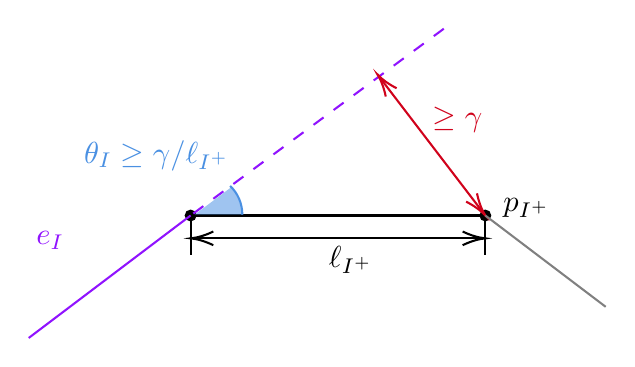
\begin{tikzpicture}[x=0.75pt,y=0.75pt,yscale=-1,xscale=1]
%uncomment if require: \path (0,300); %set diagram left start at 0, and has height of 300

%Straight Lines [id:da4824459250371491] 
\draw [color={rgb, 255:red, 0; green, 0; blue, 0 }  ,draw opacity=1 ]   (428,139.8) -- (286,139.8) ;
\draw [shift={(286,139.8)}, rotate = 180] [color={rgb, 255:red, 0; green, 0; blue, 0 }  ,draw opacity=1 ][fill={rgb, 255:red, 0; green, 0; blue, 0 }  ,fill opacity=1 ][line width=0.75]      (0, 0) circle [x radius= 2.34, y radius= 2.34]   ;
\draw [shift={(428,139.8)}, rotate = 180] [color={rgb, 255:red, 0; green, 0; blue, 0 }  ,draw opacity=1 ][fill={rgb, 255:red, 0; green, 0; blue, 0 }  ,fill opacity=1 ][line width=0.75]      (0, 0) circle [x radius= 2.34, y radius= 2.34]   ;
%Straight Lines [id:da6240195953567047] 
\draw    (426,150.8) -- (288,150.8) ;
\draw [shift={(286,150.8)}, rotate = 360] [color={rgb, 255:red, 0; green, 0; blue, 0 }  ][line width=0.75]    (10.93,-3.29) .. controls (6.95,-1.4) and (3.31,-0.3) .. (0,0) .. controls (3.31,0.3) and (6.95,1.4) .. (10.93,3.29)   ;
\draw [shift={(428,150.8)}, rotate = 180] [color={rgb, 255:red, 0; green, 0; blue, 0 }  ][line width=0.75]    (10.93,-3.29) .. controls (6.95,-1.4) and (3.31,-0.3) .. (0,0) .. controls (3.31,0.3) and (6.95,1.4) .. (10.93,3.29)   ;
%Straight Lines [id:da12589308806645683] 
\draw    (286,139.8) -- (286,158.8) ;
%Straight Lines [id:da7859420137066957] 
\draw    (428,139.8) -- (428,158.8) ;
%Straight Lines [id:da6380781281343051] 
\draw [color={rgb, 255:red, 144; green, 19; blue, 254 }  ,draw opacity=1 ]   (286,139.8) -- (208,198.8) ;
%Straight Lines [id:da42700562293346644] 
\draw [color={rgb, 255:red, 144; green, 19; blue, 254 }  ,draw opacity=1 ] [dash pattern={on 4.5pt off 4.5pt}]  (408,49.8) -- (286,139.8) ;
%Straight Lines [id:da9182056796383498] 
\draw [color={rgb, 255:red, 208; green, 2; blue, 27 }  ,draw opacity=1 ][line width=0.75]    (377.21,73.39) -- (426.79,138.22) ;
\draw [shift={(428,139.8)}, rotate = 232.59] [color={rgb, 255:red, 208; green, 2; blue, 27 }  ,draw opacity=1 ][line width=0.75]    (10.93,-3.29) .. controls (6.95,-1.4) and (3.31,-0.3) .. (0,0) .. controls (3.31,0.3) and (6.95,1.4) .. (10.93,3.29)   ;
\draw [shift={(376,71.8)}, rotate = 52.59] [color={rgb, 255:red, 208; green, 2; blue, 27 }  ,draw opacity=1 ][line width=0.75]    (10.93,-3.29) .. controls (6.95,-1.4) and (3.31,-0.3) .. (0,0) .. controls (3.31,0.3) and (6.95,1.4) .. (10.93,3.29)   ;
%Straight Lines [id:da042755669299258114] 
\draw [color={rgb, 255:red, 128; green, 128; blue, 128 }  ,draw opacity=1 ]   (428,139.8) -- (486,183.8) ;
%Shape: Pie [id:dp41789800442100455] 
\draw  [color={rgb, 255:red, 255; green, 255; blue, 255 }  ,draw opacity=0 ][fill={rgb, 255:red, 74; green, 144; blue, 226 }  ,fill opacity=0.53 ] (305.65,126.11) .. controls (305.65,126.11) and (305.65,126.11) .. (305.65,126.11) .. controls (308.72,130.21) and (310.46,134.84) .. (310.93,139.43) -- (287.87,139.43) -- cycle ;
%Shape: Arc [id:dp14809945499425647] 
\draw  [draw opacity=0] (310.93,139.43) .. controls (310.9,133.89) and (308.63,128.93) .. (305.05,125.56) -- (293.93,139.54) -- cycle ; \draw  [color={rgb, 255:red, 74; green, 144; blue, 226 }  ,draw opacity=1 ] (310.93,139.43) .. controls (310.9,133.89) and (308.63,128.93) .. (305.05,125.56) ;  

% Text Node
\draw (210,146) node [anchor=north west][inner sep=0.75pt]  [color={rgb, 255:red, 144; green, 19; blue, 254 }  ,opacity=1 ,xscale=1.1,yscale=1.1] [align=left] {$\displaystyle e_I$};
% Text Node
\draw (351,153) node [anchor=north west][inner sep=0.75pt]  [xscale=1.1,yscale=1.1] [align=left] {$\displaystyle \ell _{I^+}$};
% Text Node
\draw (435,130) node [anchor=north west][inner sep=0.75pt]  [xscale=1.1,yscale=1.1] [align=left] {$\displaystyle p_{I^+}$};
% Text Node
\draw (401,86) node [anchor=north west][inner sep=0.75pt]  [color={rgb, 255:red, 208; green, 2; blue, 27 }  ,opacity=1 ,xscale=1.1,yscale=1.1] [align=left] {$\displaystyle \geq \gamma $};
% Text Node
\draw (233,102) node [anchor=north west][inner sep=0.75pt]  [color={rgb, 255:red, 74; green, 144; blue, 226 }  ,opacity=1 ,xscale=1.1,yscale=1.1] [align=left] {$\displaystyle \theta _{I} \geq \gamma /\ell _{I^+}$};


\end{tikzpicture}